% questions.tex —— 2009 年·普通高等学校招生考试·江苏卷 · 题目内容片段（无答案）
% 由 tools/generate_projects.py 依来源总账自 2009/2009_数学真题_江苏_试题.md 生成，勿手改（改源 MD 后重跑）


\gkpart{一、填空题}

\begin{question}
\gkti{1}若复数 $z_1=4+29\mathrm i$，$z_2=6+9\mathrm i$，其中 $\mathrm i$ 是虚数单位，则复数 $(z_1-z_2)\mathrm i$ 的实部为\gkblank{}。

\end{question}
\begin{question}
\gkti{2}已知向量 $\boldsymbol a$ 和向量 $\boldsymbol b$ 的夹角为 $30^\circ$，$|\boldsymbol a|=2$，$|\boldsymbol b|=\sqrt3$，则向量 $\boldsymbol a$ 和向量 $\boldsymbol b$ 的数量积 $\boldsymbol a\cdot\boldsymbol b=$\gkblank{}。

\end{question}
\begin{question}
\gkti{3}函数 $f(x)=x^3-15x^2-33x+6$ 的单调减区间为\gkblank{}。

\Needspace{0.4\textheight}
\end{question}
\begin{question}
\gkti{4}函数 $y=A\sin(\omega x+\varphi)$（$A$，$\omega$，$\varphi$ 为常数，$A>0$，$\omega>0$）在闭区间 $[-\pi,0]$ 上的图象如图所示，则 $\omega=$\gkblank{}。
\nopagebreak[4]
\begin{center}% 2009 年江苏卷第 4 题：y=A sin(ωx+φ) 在 [−π,0] 上的图象。
% 来源 PDF：普通高考/2009/2009江苏.pdf
% SHA-256：64e417d45911d88d77c047a419dcc259e7c7dc779c79d20df2092755c96a4501
% 原页：2009江苏.pdf 第 1 页（A3 三栏）第 1 栏，书页码 531。
% 绘制依据：按原页曲线在 [−π,0] 上与 x 轴依次交于 −π、−2π/3、−π/3、0，
%   在 −π/2 处取最大值，在 −5π/6、−π/6 处取最小值；取 A=1、φ=0 绘 y=sin3x。
\begin{tikzpicture}[x=1.15cm, y=1.15cm, semithick, every node/.style={inner sep=1.6pt}]
  \draw[->,>=stealth] (-3.55,0) -- (0.75,0) node[below] {$x$};
  \draw[->,>=stealth] (0,-1.55) -- (0,1.75) node[right] {$y$};

  \draw[domain=-3.14159:0, samples=160, smooth] plot (\x,{sin(3*\x r)});

  \node[below left] at (-3.14159,0) {$-\pi$};
  \node[above] at (-2.42,0.06) {$-\dfrac{2\pi}3$};
  \node[above] at (-0.70,0.06) {$-\dfrac{\pi}3$};
  \node[below right] at (0.06,-0.05) {$O$};
\end{tikzpicture}
\end{center}
\nopagebreak[4]
\end{question}
\begin{question}
\gkti{5}现有 $5$ 根竹竿，它们的长度（单位：m）分别为 $2.5$，$2.6$，$2.7$，$2.8$，$2.9$，若从中一次随机抽取 $2$ 根竹竿，则它们的长度恰好相差 $0.3$ m 的概率为\gkblank{}。

\end{question}
\begin{question}
\gkti{6}某校甲、乙两个班级各有 $5$ 名编号为 $1$，$2$，$3$，$4$，$5$ 的学生进行投篮练习，每人投 $10$ 次，投中的次数如下表：

\begin{center}
\begin{tabular}{llllll}
\toprule
学生 & 1 号 & 2 号 & 3 号 & 4 号 & 5 号 \\
\midrule
甲班 & 6 & 7 & 7 & 8 & 7 \\
乙班 & 6 & 7 & 6 & 7 & 9 \\
\bottomrule
\end{tabular}
\end{center}

则以上两组数据的方差中较小的一个为 $s^2=$\gkblank{}。

\Needspace{0.4\textheight}
\end{question}
\begin{question}
\gkti{7}如图是一个算法的流程图，最后输出的 $W=$\gkblank{}。
\nopagebreak[4]
\begin{center}% 2009 年江苏卷第 7 题：求 W 的算法流程图。
% 来源 PDF：普通高考/2009/2009江苏.pdf
% SHA-256：64e417d45911d88d77c047a419dcc259e7c7dc779c79d20df2092755c96a4501
% 原页：2009江苏.pdf 第 1 页（A3 三栏）第 1 栏，书页码 531。
% 绘制依据：按原页流程：开始 → S←0 → T←1 → S←T²−S → 判断 S≥10 →
%   N 时 T←T+2 回环 → Y 时 W←S+T → 输出 W → 结束。
\begin{tikzpicture}[node distance=0.55cm, semithick, every node/.style={inner sep=3pt},
  box/.style={draw, minimum width=2.0cm, minimum height=0.55cm},
  io/.style={draw, trapezium, trapezium left angle=70, trapezium right angle=110,
             minimum width=2.3cm, minimum height=0.55cm},
  dec/.style={draw, diamond, aspect=1.9, inner sep=1pt}]

  \node[box, rounded corners=2pt] (start) {开始};
  \node[box, below=of start] (s0) {$S\leftarrow0$};
  \node[box, below=of s0] (t1) {$T\leftarrow1$};
  \node[dec, below=0.6cm of t1, minimum width=2.4cm, minimum height=0.95cm] (assign)
    {$S\leftarrow T^2-S$};
  \node[dec, below=0.55cm of assign, minimum width=1.9cm, minimum height=0.95cm] (test)
    {$S\geqslant10$};
  \node[box, below=0.65cm of test] (w) {$W\leftarrow S+T$};
  \node[io, below=of w] (out) {输出 $W$};
  \node[box, rounded corners=2pt, below=of out] (end) {结束};
  \node[box, right=1.5cm of assign] (inc) {$T\leftarrow T+2$};

  \draw[->,>=stealth] (start) -- (s0);
  \draw[->,>=stealth] (s0) -- (t1);
  \draw[->,>=stealth] (t1) -- (assign);
  \draw[->,>=stealth] (assign) -- (test);
  \draw[->,>=stealth] (test) -- node[left] {Y} (w);
  \draw[->,>=stealth] (w) -- (out);
  \draw[->,>=stealth] (out) -- (end);
  \draw[->,>=stealth] (test.east) -- node[above] {N} ++(0.30,0) -| (inc.south);
  \draw (inc.north) -- ++(0,0.65) -| ($(t1.south)!0.45!(assign.north)$);
\end{tikzpicture}
\end{center}
\nopagebreak[4]
\end{question}
\begin{question}
\gkti{8}在平面上，若两个正三角形的边长的比为 $1:2$，则它们的面积比为 $1:4$，类似地，在空间内，若两个正四面体的棱长的比为 $1:2$，则它们的体积比为\gkblank{}。

\end{question}
\begin{question}
\gkti{9}在平面直角坐标系 $xOy$ 中，点 $P$ 在曲线 $C$：$y=x^3-10x+3$ 上，且在第二象限内，已知曲线 $C$ 在点 $P$ 处的切线的斜率为 $2$，则点 $P$ 的坐标为\gkblank{}。

\end{question}
\begin{question}
\gkti{10}已知 $a=\dfrac{\sqrt5-1}{2}$，函数 $f(x)=a^x$，若实数 $m$、$n$ 满足 $f(m)>f(n)$，则 $m$、$n$ 的大小关系为\gkblank{}。

\end{question}
\begin{question}
\gkti{11}已知集合 $A=\{x\mid \log_2x\leqslant2\}$，$B=(-\infty,a)$，若 $A\subseteq B$，则实数 $a$ 的取值范围是 $(c,+\infty)$，其中 $c=$\gkblank{}。

\end{question}
\begin{question}
\gkti{12}设 $\alpha$ 和 $\beta$ 为不重合的两个平面，给出下列命题：

（1）若 $\alpha$ 内的两条相交直线分别平行于 $\beta$ 内的两条直线，则 $\alpha$ 平行于 $\beta$；

（2）若 $\alpha$ 外一条直线 $l$ 与 $\alpha$ 内的一条直线平行，则 $l$ 和 $\alpha$ 平行；

（3）设 $\alpha$ 和 $\beta$ 相交于直线 $l$，若 $\alpha$ 内有一条直线垂直于 $l$，则 $\alpha$ 和 $\beta$ 垂直；

（4）直线 $l$ 与 $\alpha$ 垂直的充分必要条件是 $l$ 与 $\alpha$ 内的两条直线垂直。

上面命题中，真命题的序号\gkblank{}。（写出所有真命题的序号）

\Needspace{0.4\textheight}
\end{question}
\begin{question}
\gkti{13}如图，在平面直角坐标系 $xOy$ 中，$A_1$，$A_2$，$B_1$，$B_2$ 为椭圆 $\dfrac{x^2}{a^2}+\dfrac{y^2}{b^2}=1$（$a>b>0$）的四个顶点，$F$ 为其右焦点，直线 $A_1B_2$ 与直线 $B_1F$ 相交于点 $T$，线段 $OT$ 与椭圆的交点 $M$ 恰为线段 $OT$ 的中点，则该椭圆的离心率为\gkblank{}。
\nopagebreak[4]
\begin{center}% 2009 年江苏卷第 13 题：椭圆的四个顶点、右焦点 F、交点 T 与中点 M。
% 来源 PDF：普通高考/2009/2009江苏.pdf
% SHA-256：64e417d45911d88d77c047a419dcc259e7c7dc779c79d20df2092755c96a4501
% 原页：2009江苏.pdf 第 1 页（A3 三栏）第 2 栏，书页码 531。
% 绘制依据：按原页画椭圆 A1A2B2B1、右焦点 F、直线 A1B2 与 B1F 的交点 T，
%   以及 OT 的中点 M（落在椭圆上）；示意取 a=2.6，b≈2.487，e=2√7−5。
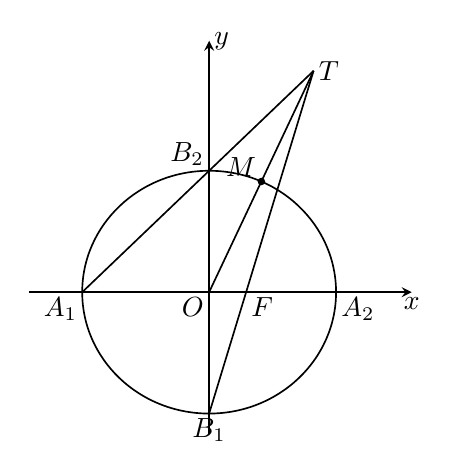
\begin{tikzpicture}[scale=0.62, semithick, every node/.style={inner sep=1.6pt}]
  \draw (0,0) ellipse [x radius=2.6, y radius=2.4868];

  \coordinate (A1) at (-2.6,0);
  \coordinate (A2) at (2.6,0);
  \coordinate (B1) at (0,-2.4868);
  \coordinate (B2) at (0,2.4868);
  \coordinate (F) at (0.7579,0);
  \coordinate (T) at (2.1394,4.5335);
  \coordinate (M) at (1.0697,2.2668);

  \draw[->,>=stealth] (-3.7,0) -- (4.15,0) node[below] {$x$};
  \draw[->,>=stealth] (0,-2.9) -- (0,5.15) node[right] {$y$};

  \draw (A1) -- (T);
  \draw (B1) -- (T);
  \draw (0,0) -- (T);

  \fill (M) circle (2.2pt);

  \node[below left] at (A1) {$A_1$};
  \node[below right] at (A2) {$A_2$};
  \node[below] at (B1) {$B_1$};
  \node[above left] at (B2) {$B_2$};
  \node[below right] at (F) {$F$};
  \node[right] at (T) {$T$};
  \node[above left] at (M) {$M$};
  \node[below left] at (0,0) {$O$};
\end{tikzpicture}
\end{center}
\nopagebreak[4]
\end{question}
\begin{question}
\gkti{14}设 $\{a_n\}$ 是公比为 $q$ 的等比数列，$|q|>1$，令 $b_n=a_n+1$（$n=1,2,\cdots$），若数列 $\{b_n\}$ 有连续四项在集合 $\{-53,-23,19,37,82\}$ 中，则 $6q=$\gkblank{}。

\end{question}
\gkpart{二、解答题}

\begin{question}
\gkti{15}设向量 $\boldsymbol a=(4\cos\alpha,\sin\alpha)$，$\boldsymbol b=(\sin\beta,4\cos\beta)$，$\boldsymbol c=(\cos\beta,-4\sin\beta)$。

（1）若 $\boldsymbol a$ 与 $\boldsymbol b-2\boldsymbol c$ 垂直，求 $\tan(\alpha+\beta)$ 的值；

（2）求 $|\boldsymbol b+\boldsymbol c|$ 的最大值；

（3）若 $\tan\alpha\tan\beta=16$，求证：$\boldsymbol a\parallel\boldsymbol b$。

\Needspace{0.4\textheight}
\end{question}
\begin{question}
\gkti{16}如图，在直三棱柱 $ABC-A_1B_1C_1$ 中，$E$、$F$ 分别是 $A_1B$、$A_1C$ 的中点，点 $D$ 在 $B_1C_1$ 上，$A_1D\perp B_1C$。求证：

（1）$EF\parallel$ 平面 $ABC$；

（2）平面 $A_1FD\perp$ 平面 $BB_1C_1C$。
\nopagebreak[4]
\begin{center}% 2009 年江苏卷第 16 题：直三棱柱 ABC−A1B1C1，E、F 为 A1B、A1C 中点，D 在 B1C1 上。
% 来源 PDF：普通高考/2009/2009江苏.pdf
% SHA-256：64e417d45911d88d77c047a419dcc259e7c7dc779c79d20df2092755c96a4501
% 原页：2009江苏.pdf 第 1 页（A3 三栏）第 3 栏，书页码 531。
% 绘制依据：按原页斜投影；被遮挡的 AC 与 A1B1 用虚线，其余实线；
%   E 在 A1B 上、F 在 A1C 上，D 在 B1C1 上，A1D 连实线。
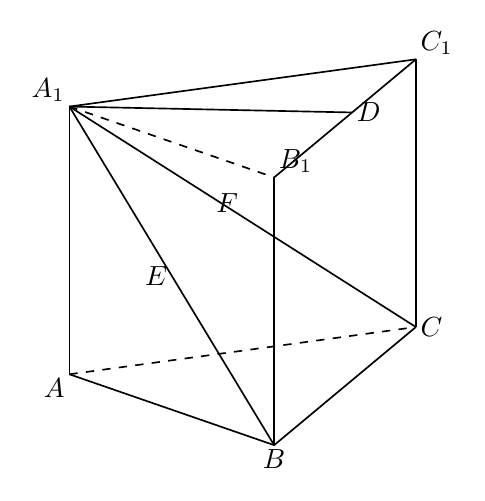
\begin{tikzpicture}[scale=1.0, semithick, every node/.style={inner sep=1.4pt}]
  \coordinate (A) at (0,0);
  \coordinate (A1) at (0,3.4);
  \coordinate (B) at (2.6,-0.9);
  \coordinate (B1) at (2.6,2.5);
  \coordinate (C) at (4.4,0.6);
  \coordinate (C1) at (4.4,4.0);
  \coordinate (D) at (3.59,3.325);
  \coordinate (E) at (1.3,1.25);
  \coordinate (F) at (2.2,2.0);

  % 前面与可见棱
  \draw (A) -- (B) -- (C);
  \draw (A) -- (A1);
  \draw (B) -- (B1);
  \draw (C) -- (C1);
  \draw (A1) -- (C1);
  \draw (B1) -- (C1);
  % 面内连线
  \draw (A1) -- (B);
  \draw (A1) -- (C);
  \draw (A1) -- (D);

  % 被遮挡的棱
  \draw[dashed] (A) -- (C);
  \draw[dashed] (A1) -- (B1);

  \node[above left] at (A1) {$A_1$};
  \node[above right] at (C1) {$C_1$};
  \node[above right] at (B1) {$B_1$};
  \node[right] at (D) {$D$};
  \node[left] at (E) {$E$};
  \node[above left] at (F) {$F$};
  \node[below left] at (A) {$A$};
  \node[right] at (C) {$C$};
  \node[below] at (B) {$B$};
\end{tikzpicture}
\end{center}
\nopagebreak[4]
\end{question}
\begin{question}
\gkti{17}设 $\{a_n\}$ 是公差不为零的等差数列，$S_n$ 为其前 $n$ 项和，满足 $a_2^2+a_3^2=a_4^2+a_5^2$，$S_7=7$。

（1）求数列 $\{a_n\}$ 的通项公式及前 $n$ 项和 $S_n$；

（2）试求所有的正整数 $m$，使得 $\dfrac{a_ma_{m+1}}{a_{m+2}}$ 为数列 $\{a_n\}$ 中的项。

\Needspace{0.4\textheight}
\end{question}
\begin{question}
\gkti{18}在平面直角坐标系 $xOy$ 中，已知圆 $C_1$ 的方程为 $(x+3)^2+(y-1)^2=4$，圆 $C_2$ 的方程为 $(x-4)^2+(y-5)^2=4$。

（1）若直线 $l$ 过点 $A(4,0)$，且被圆 $C_1$ 截得的弦长为 $2\sqrt3$，求直线 $l$ 的方程；

（2）设 $P$ 为平面上的点，满足：存在过点 $P$ 的无穷多对互相垂的直线 $l_1$ 和 $l_2$，它们分别与圆 $C_1$ 和圆 $C_2$ 相交，且直线 $l_1$ 被圆 $C_1$ 截得的弦长与直线 $l_2$ 被圆 $C_2$ 截得的弦长相等，试求所有满足条件的点 $P$ 的坐标。
\nopagebreak[4]
\begin{center}% 2009 年江苏卷第 18 题：圆 C1:(x+3)²+(y−1)²=4 与圆 C2:(x−4)²+(y−5)²=4。
% 来源 PDF：普通高考/2009/2009江苏.pdf
% SHA-256：64e417d45911d88d77c047a419dcc259e7c7dc779c79d20df2092755c96a4501
% 原页：2009江苏.pdf 第 1 页（A3 三栏）第 3 栏，书页码 531。
% 绘制依据：按原页坐标画两圆（半径均为 2）、坐标轴、圆心与点 A(4,0)。
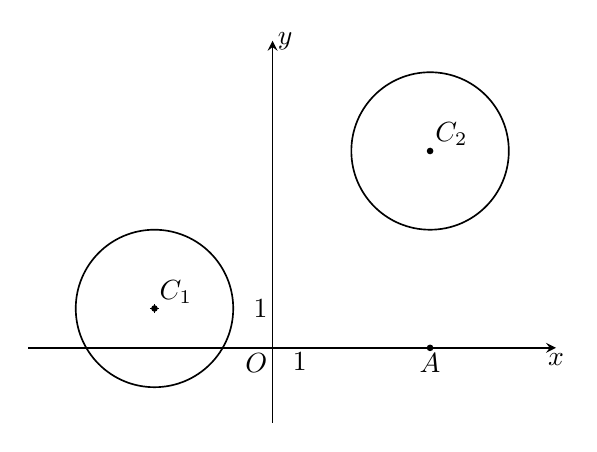
\begin{tikzpicture}[scale=0.5, semithick, every node/.style={inner sep=1.6pt}]
  \draw[->,>=stealth] (-6.2,0) -- (7.2,0) node[below] {$x$};
  \draw[->,>=stealth] (0,-1.9) -- (0,7.8) node[right] {$y$};

  \draw (-3,1) circle [radius=2];
  \draw (4,5) circle [radius=2];

  \fill (-3,1) circle (2.4pt);
  \fill (4,5) circle (2.4pt);
  \fill (4,0) circle (2.4pt);

  \draw (-3,1) ++(-0.12,0) -- ++(0.24,0);
  \draw (-3,1) ++(0,-0.12) -- ++(0,0.24);

  \node[above right] at (-3,1) {$C_1$};
  \node[above right] at (4,5) {$C_2$};
  \node[below] at (4,0) {$A$};
  \node[below left] at (0,0) {$O$};
  \node[below left] at (1,0) {$1$};
  \node[left] at (0,1) {$1$};
\end{tikzpicture}
\end{center}
\nopagebreak[4]
\end{question}
\begin{question}
\gkti{19}按照某学者的理论，假设一个人生产某产品单件成本为 $a$ 元，如果他卖出该产品的单价为 $m$ 元，则他的满意度为 $\dfrac{m}{m+a}$；如果他买进该产品的单价为 $n$ 元，则他的满意度为 $\dfrac{n}{n+a}$。如果一个人对两种交易（卖出或买进）的满意度分别为 $h_1$ 和 $h_2$，则他对这两种交易的综合满意度为 $\sqrt{h_1h_2}$。

现假设甲生产 $A$、$B$ 两种产品的单件成本分别为 $12$ 元和 $5$ 元，乙生产 $A$、$B$ 两种产品的单件成本分别为 $3$ 元和 $20$ 元，设产品 $A$、$B$ 的单价分别为 $m_A$ 元和 $m_B$ 元，甲买进 $A$ 与卖出 $B$ 的综合满意度为 $h_{\text{\text{甲}}}$，乙卖出 $A$ 与买进 $B$ 的综合满意度为 $h_{\text{\text{乙}}}$。

（1）求 $h$ 和 $h_{\text{\text{乙}}}$ 关于 $m_A$、$m_B$ 的表达式；当 $m_A=\dfrac35m_B$ 时，求证：$h_{\text{\text{甲}}}=h_{\text{\text{乙}}}$；

（2）设 $m_A=\dfrac35m_B$，当 $m_A$、$m_B$ 分别为多少时，甲、乙两人的综合满意度均最大？最大的综合满意度为多少？

（3）记（2）中最大的综合满意度为 $h_0$，试问能否适当选取 $m_A$、$m_B$ 的值，使得 $h_{\text{\text{甲}}}\geqslant h_0$ 和 $h_{\text{\text{乙}}}\geqslant h_0$ 同时成立，但等号不同时成立？试说明理由。

\end{question}
\begin{question}
\gkti{20}设 $a$ 为实数，函数 $f(x)=2x^2+(x-a)|x-a|$。

（1）若 $f(0)\geqslant1$，求 $a$ 的取值范围；

（2）求 $f(x)$ 的最小值；

（3）设函数 $h(x)=f(x)$，$x\in(a,+\infty)$，直接写出（不需给出演算步骤）不等式 $h(x)\geqslant1$ 的解集。

\end{question}
\gkpart{三、附加题}

\Needspace{0.4\textheight}
\begin{question}
\gkti{21}四选二。

【A】如图，在四边形 $ABCD$ 中，$\triangle ABC\cong\triangle BAD$。求证：$AB\parallel CD$。
\nopagebreak[4]
\begin{center}% 2009 年江苏卷第 21A 题：四边形 ABCD，△ABC≌△BAD。
% 来源 PDF：普通高考/2009/2009江苏.pdf
% SHA-256：64e417d45911d88d77c047a419dcc259e7c7dc779c79d20df2092755c96a4501
% 原页：2009江苏.pdf 第 2 页（A3 三栏）第 2 栏，书页码 532。
% 绘制依据：按原页画四边形 ABCD（A 左下、B 右下、D 左上、C 右上）及对角线 AC、BD。
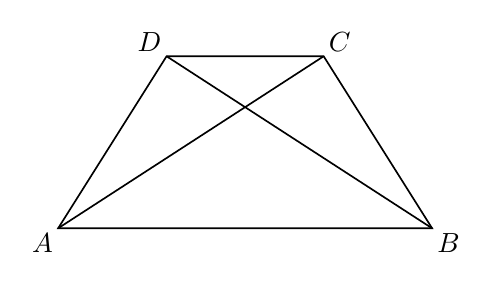
\begin{tikzpicture}[scale=0.95, semithick, every node/.style={inner sep=1.6pt}]
  \coordinate (A) at (0,0);
  \coordinate (B) at (5,0);
  \coordinate (C) at (3.55,2.3);
  \coordinate (D) at (1.45,2.3);

  \draw (A) -- (B) -- (C) -- (D) -- cycle;
  \draw (A) -- (C);
  \draw (B) -- (D);

  \node[below left] at (A) {$A$};
  \node[below right] at (B) {$B$};
  \node[above right] at (C) {$C$};
  \node[above left] at (D) {$D$};
\end{tikzpicture}
\end{center}
\nopagebreak[4]
【B】求矩阵 $\boldsymbol A=\begin{bmatrix}3&2\\2&1\end{bmatrix}$ 的逆矩阵。

【C】已知曲线 $C$ 的参数方程为 $\begin{cases}x=\sqrt t-\dfrac1{\sqrt t},\\ y=3\left(t+\dfrac1t\right),\end{cases}$（$t$ 为参数，$t>0$），求曲线 $C$ 的普通方程。

【D】设 $a\geqslant b>0$，求证：$3a^3+2b^3\geqslant3a^2b+2ab^2$。

\Needspace{0.4\textheight}
\end{question}
\begin{question}
\gkti{22}在平面直角坐标系 $xOy$ 中，抛物线 $C$ 的顶点在原点，经过点 $A(2,2)$，其焦点 $F$ 在 $x$ 轴上。

（1）求抛物线 $C$ 的标准方程；

（2）求过点 $F$，且与直线 $OA$ 垂直的直线的方程；

（3）设过点 $M(m,0)$（$m>0$）的直线交抛物线 $C$ 于 $D$、$E$ 两点，$ME=2DM$，记 $D$ 和 $E$ 两点间的距离为 $f(m)$，求 $f(m)$ 关于 $m$ 的表达式。
\nopagebreak[4]
\begin{center}% 2009 年江苏卷第 22 题：抛物线 y²=2x 与点 A(2,2)、直线 OA。
% 来源 PDF：普通高考/2009/2009江苏.pdf
% SHA-256：64e417d45911d88d77c047a419dcc259e7c7dc779c79d20df2092755c96a4501
% 原页：2009江苏.pdf 第 2 页（A3 三栏）第 3 栏，书页码 532。
% 绘制依据：按原页画坐标轴、抛物线两支、点 A 及线段 OA，并在两轴标出单位刻度 1。
\begin{tikzpicture}[x=0.95cm, y=0.95cm, semithick, every node/.style={inner sep=1.6pt}]
  \draw[->,>=stealth] (-0.7,0) -- (5.6,0) node[below] {$x$};
  \draw[->,>=stealth] (0,-3.4) -- (0,3.5) node[right] {$y$};

  \draw[domain=-3.15:3.15, samples=140, smooth, variable=\t]
    plot ({\t*\t/2}, \t);

  \draw (0,0) -- (2,2);
  \fill (2,2) circle (2.2pt);
  \node[above right] at (2,2) {$A$};

  \draw (1,0) ++(0,-0.09) -- ++(0,0.18);
  \draw (0,1) ++(-0.09,0) -- ++(0.18,0);
  \node[below] at (1,0) {$1$};
  \node[left] at (0,1) {$1$};
  \node[below left] at (0,0) {$O$};
\end{tikzpicture}
\end{center}
\nopagebreak[4]
\end{question}
\begin{question}
\gkti{23}对于正整数 $n\geqslant2$，用 $T_n$ 表示关于 $x$ 的一元二次方程 $x^2+2ax+b=0$ 有实数根的有序数组 $(a,b)$ 的组数，其中 $a,b\in\{1,2,\cdots,n\}$（$a$ 和 $b$ 可以相等）；对于随机选取的 $a,b\in\{1,2,\cdots,n\}$（$a$ 和 $b$ 可以相等），记 $P_n$ 为关于 $x$ 的一元二次方程 $x^2+2ax+b=0$ 有实数根的概率。

（1）求 $T_{n^2}$ 和 $P_{n^2}$；

（2）求证：对任意正整数 $n\geqslant2$，有 $P_n>1-\dfrac1{\sqrt n}$。

\end{question}